% !TEX TS-program = xelatex
% !BIB program = bibtex
% !TeX spellcheck = ru_RU

% About magic macros see also
% https://tex.stackexchange.com/questions/78101/

% По умолчанию используется шрифт 14 размера.
% Если Вы не влезаете в лимит страниц и нужен 12-й шрифт,
% то уберите опцию [14pt]

\documentclass[14pt, russian]{matmex-diploma-custom}

% !TeX spellcheck = ru_RU
% !TEX root = vkr.tex
% Опциональные добавления используемых пакетов. Вполне может быть, что они вам не понадобятся, но в шаблоне приведены примеры их использования.
\usepackage{tikz} % Мощный пакет для создание рисунков, однако может очень сильно замедлять компиляцию
\usetikzlibrary{decorations.pathreplacing,calc,shapes,positioning,tikzmark}

% Библиотека для TikZ, которая генерирует отдельные файлы для каждого рисунка
% Позволяет ускорить компиляцию, однако имеет свои ограничения
% Например, ломает пример выделения кода в листинге из шаблона
% \usetikzlibrary{external}
% \tikzexternalize[prefix=figures/]

\newcounter{tmkcount}

\tikzset{
    use tikzmark/.style={
            remember picture,
            overlay,
            execute at end picture={
                    \stepcounter{tmkcount}
                },
        },
    tikzmark suffix={-\thetmkcount}
}

\usepackage{booktabs} % Пакет для верстки "более книжных" таблиц, вполне годится для оформления результатов
% В шаблоне есть команда \multirowcell, которой нужен этот пакет.
\usepackage{multirow}
\usepackage{siunitx} % для таблиц с единицами измерений
\usepackage{algpseudocode}
\usepackage{algorithm}
\usepackage{algorithmicx}
\usepackage[export]{adjustbox}


% \DeclareFloatingEnvironment[placement={!ht},name=]{listing}
% \captionsetup[listing]{labelformat=parens}
% \sidecaptionvpos{listing}{c}
% \makeatletter
% \makeatother

% Для названий стоит использовать \textsc{}
\newcommand{\OCaml}{\textsc{OCaml}}
\newcommand{\miniKanren}{\textsc{miniKanren}}
\newcommand{\BibTeX}{\textsc{BibTeX}}
\newcommand{\vsharp}{\textsc{V$\sharp$}}
\newcommand{\fsharp}{\textsc{F$\sharp$}}
\newcommand{\csharp}{\textsc{C\#}}
\newcommand{\GitHub}{\textsc{GitHub}}
\newcommand{\SMT}{\textsc{SMT}}

\definecolor{eclipseGreen}{RGB}{63,127,95}
% \lstdefinelanguage{ocaml}{
% keywords={@type, function, fun, let, in, match, with, when, class, type,
% nonrec, object, method, of, rec, repeat, until, while, not, do, done, as, val, inherit, and,
% new, module, sig, deriving, datatype, struct, if, then, else, open, private, virtual, include, success, failure,
% lazy, assert, true, false, end},
% sensitive=true,
% commentstyle=\small\itshape\ttfamily,
% keywordstyle=\ttfamily\bfseries, %\underbar,
% identifierstyle=\ttfamily,
% basewidth={0.5em,0.5em},
% columns=fixed,
% fontadjust=true,
% literate={->}{{$\to$}}3 {===}{{$\equiv$}}1 {=/=}{{$\not\equiv$}}1 {|>}{{$\triangleright$}}3 {\\/}{{$\vee$}}2 {/\\}{{$\wedge$}}2 {>=}{{$\ge$}}1 {<=}{{$\le$}} 1,
% morecomment=[s]{(*}{*)}
% }

\makeatletter
\@ifclassloaded{beamer}{
    %%% Обязательные пакеты
    %% Beamer
    \usepackage{beamerthemesplit}
    \usetheme{SPbGU}
    \beamertemplatenavigationsymbolsempty
    \usepackage{appendixnumberbeamer}

    %% Локализация
    \usepackage{fontspec}
    \setmainfont{CMU Serif}
    \setsansfont{CMU Sans Serif}
    \setmonofont{CMU Typewriter Text}
    %\setmonofont{Fira Code}[Contextuals=Alternate,Scale=0.9]
    %\setmonofont{Inconsolata}
    \usepackage{polyglossia}
    \setmainlanguage{russian}
    \setotherlanguage{english}

    %% Графика
    \usepackage{pdfpages} % Позволяет вставлять многостраничные pdf документы в текст

    % Математические окружения с русским названием
    \newtheorem{rutheorem}{Теорема}
    \newtheorem{ruproof}{Доказательство}
    \newtheorem{rudefinition}{Определение}
    \newtheorem{rulemma}{Лемма}
    \usepackage{fancyvrb}
}
{}
\makeatother

\usepackage[autostyle]{csquotes} % Правильные кавычки в зависимости от языка
\usepackage{totcount}
\usepackage{setspace}
\usepackage{amsmath, amsfonts, amssymb, amsthm, mathtools} % "Адекватная" работа с математикой в LaTeX

\usepackage{url}
\usepackage[
  backend=biber,
  style=gost-numeric,
  sorting=none,
  autolang=other
]{biblatex}
\addbibresource{references.bib}

\begin{document}

% !TeX spellcheck = ru_RU
% !TEX root = vkr.tex

%% Если что-то забыли, при компиляции будут ошибки Undefined control sequence \my@title@<что забыли>@ru
%% Если англоязычная титульная страница не нужна, то ее можно просто удалить.
\filltitle{ru}{
    %% Актуально только для курсовых/практик. ВКР защищаются не на кафедре а в ГЭК по направлению,
    %%   и к моменту защиты вы будете уже не в группе.
    chair              = {Кафедра системного программирования },
    group              = {23.Б08-мм},
    %
    %% Макрос filltitle ненавидит пустые строки, поэтому обязателен хотя бы символ комментария на строке
    %% Актуально всем.
    title = { 
       Исследование производительности умножения матриц на графических ускорителях от Imagination Technologies
    },
    %
    %% Здесь указывается тип работы. Возможные значения:
    %%   production - производственная практика;
    %%   coursework - отчёт по курсовой работе (ОБРАТИТЕ ВНИМАНИЕ, у техпрога и ПИ нет курсовых, только практики);
    %%   practice - отчёт по учебной практике;
    %%   prediploma - отчёт по преддипломной практике;
    %%   master - ВКР магистра;
    %%   bachelor - ВКР бакалавра.
    type               = {practice},
    %
    %% Здесь указывается вид работы. От вида работы зависят критерии оценивания.
    %%   solution - «Решение». Обучающемуся поручили найти способ решения проблемы в области разработки программного обеспечения или теоретической информатики с учётом набора ограничений.
    %%   experiment - «Эксперимент». Обучающемуся поручили изучить возможности, достоинства и недостатки новой технологии, платформы, языка и т. д. на примере какой-то задачи.
    %%   production - «Производственное задание». Автору поручили реализовать потенциально полезное программное обеспечение.
    %%   comparison - «Сравнение». Обучающемуся поручили сравнить несколько существующих продуктов и/или подходов.
    %%   theoretical - «Теоретическое исследование». Автору поручили доказать какое-то утверждение, исследовать свойства алгоритма и т.п., при этом не требуя написания кода.
    kind               = {solution},
    %
    author             = {Пучкин Станислав Андреевич},
    %
    %% Актуально только для ВКР. Указывается код и название направления подготовки. Типичные примеры:
    %%   02.03.03 \enquote{Математическое обеспечение и администрирование информационных систем}
    %%   02.04.03 \enquote{Математическое обеспечение и администрирование информационных систем}
    %%   09.03.04 \enquote{Программная инженерия}
    %%   09.04.04 \enquote{Программная инженерия}
    %% Те, что с 03 в середине --- бакалавриат, с 04 --- магистратура.
    specialty          = {02.03.03 \enquote{Математическое обеспечение и администрирование информационных систем}},
    %
    %% Актуально только для ВКР. Указывается шифр и название образовательной программы. Типичные примеры:
    %%   СВ.5162.2020 \enquote{Технологии программирования}
    %%   СВ.5080.2020 \enquote{Программная инженерия}
    %%   ВМ.5665.2022 \enquote{Математическое обеспечение и администрирование информационных систем}
    %%   ВМ.5666.2022 \enquote{Программная инженерия}
    %% Шифр и название программы можно посмотреть в учебном плане, по которому вы учитесь.
    %% СВ.* --- бакалавриат, ВМ.* --- магистратура. В конце --- год поступления (не обязательно ваш, если вы были в академе/вылетали).
    programme          = {СВ.5162.2020 \enquote{Технологии программирования}},
    %
    %% Актуально всем.
    %% Должно умещаться в одну строчку, допускается использование сокращений, но без переусердствования,
    %% короткая строка с большим количеством сокращений выглядит странно
    %supervisorPosition = {проф. кафeдры системного программирования, д.ф.-м.н.,}, % Терехов А. Н.
    %supervisorPosition = {ст. преподаватель кафедры ИАС, к.~ф.-м.~н. (если есть),}, % Смирнов К. К.
    supervisorPosition = {доцент кафедры системного программирования, к.~ф.-м.~н.,},
    supervisor         = {Григорьев С. В.},
    %
    %% Актуально только для практик и курсовых. Если консультанта нет или он совпадает с научником, закомментировать или удалить вовсе.
    % consultantPosition = {должность, ООО \enquote{Место работы}, степень  (если есть),},
    % consultant         = {Консультант~К.~К.},
    %
    %% Актуально только для ВКР.
    reviewerPosition   = {должность, ООО \enquote{Место работы}, степень (если есть),},
    reviewer           = {Рецензент~Р.~Р.},
}

% Английский титульник нужен только для ВКР, остальные виды работ могут его смело игнорировать.
\filltitle{en}{
    chair              = {Advisor's chair},
    group              = {ХХ.BХХ-mm},
    title              = {Template for SPbU qualification works},
    type               = {bachelor},
    author             = {FirstName Surname},
    %
    %% Possible choices:
    %%   02.03.03 \foreignquote{english}{Software and Administration of Information Systems}
    %%   02.04.03 \foreignquote{english}{Software and Administration of Information Systems}
    %%   09.03.04 \foreignquote{english}{Software Engineering}
    %%   09.04.04 \foreignquote{english}{Software Engineering}
    %% Те, что с 03 в середине --- бакалавриат, с 04 --- магистратура.
    specialty          = {02.03.03 \foreignquote{english}{Software and Administration of Information Systems}},
    %
    %% Possible choices:
    %%   СВ.5162.2020 \foreignquote{english}{Programming Technologies}
    %%   СВ.5080.2020 \foreignquote{english}{Software Engineering}
    %%   ВМ.5665.2022 \foreignquote{english}{Software and Administration of Information Systems}
    %%   ВМ.5666.2022 \foreignquote{english}{Software Engineering}
    programme          = {СВ.5162.2020 \foreignquote{english}{Programming Technologies}},
    %
    %% Note that common title translations are:
    %%   кандидат наук --- C.Sc. (NOT Ph.D.)
    %%   доктор ... наук --- Sc.D.
    %%   доцент --- docent (NOT assistant/associate prof.)
    %%   профессор --- prof.
    supervisorPosition = {Sc.D, prof.},
    supervisor         = {S.S. Supervisor},
    %
    consultantPosition = {position at \foreignquote{english}{Company}, degree if present},
    consultant         = {C.C. Consultant},
    %
    reviewerPosition   = {position at \foreignquote{english}{Company}, degree if present},
    reviewer           = {R.R. Reviewer},
}

\maketitle
\setcounter{tocdepth}{2}
\tableofcontents

% !TeX spellcheck = ru_RU
% !TEX root = vkr.tex

\section*{Введение}
\thispagestyle{withCompileDate}

Операции линейной алгебры составляют вычислительное ядро многих современных приложений: от машинного обучения и компьютерного зрения до научных расчётов и финансового моделирования. Среди них операция умножения матриц общего вида (GEMM, General Matrix Multiply) является наиболее критичной с точки зрения производительности, поскольку её эффективная реализация определяет скорость работы алгоритмов свёрточных нейронных сетей, итерационных решателей систем линейных уравнений и многих других методов.

Для ускорения таких вычислений активно используются графические процессоры (GPU) и специализированные ускорители, обладающие массивно-параллельной архитектурой. Однако разработка эффективного программного обеспечения для GPU осложняется разнообразием аппаратных платформ: различные производители (NVIDIA, AMD, Intel) предлагают собственные архитектуры и программные интерфейсы. Наиболее распространённый API для GPU вычислений --- CUDA~\cite{nickolls2008cuda} --- является проприетарной технологией NVIDIA и не поддерживается на устройствах других производителей.

Альтернативой проприетарным решениям служит открытый стандарт OpenCL~\cite{opencl_spec} (Open Computing Language) --- кросс-платформенный фреймворк для параллельного программирования, позволяющий разрабатывать приложения, исполняемые на различных вычислительных устройствах независимо от производителя. OpenCL обеспечивает переносимость кода и абстрагирование от специфики аппаратной архитектуры, что делает его привлекательным выбором для создания кросс-вендорных решений.

В последние годы особое внимание привлекает открытая архитектура набора команд RISC-V~\cite{waterman2014risc}. В отличие от проприетарных архитектур x86 и ARM, RISC-V является полностью открытой спецификацией, доступной для использования, модификации и расширения без лицензионных отчислений. Открытость RISC-V стимулирует появление новых процессоров и ускорителей, в том числе для встраиваемых систем и одноплатных компьютеров. Экосистема RISC-V активно развивается: появляются производительные многоядерные процессоры, поддержка векторных расширений и реализации OpenCL, что открывает возможности для высокопроизводительных вычислений на этой архитектуре.

Однако эффективность существующих библиотек линейной алгебры на платформах RISC-V остаётся малоисследованной областью. Различия в архитектуре процессоров, особенности реализации инструкций, размеры кэш-памяти и характеристики подсистемы памяти могут существенно влиять на производительность различных алгоритмических подходов к реализации GEMM. Понимание этих особенностей критически важно для разработки эффективных вычислительных приложений на RISC-V платформах.

Библиотека MyGEMM~\cite{nugteren2018mygemm} предоставляет набор реализаций алгоритма умножения матриц для OpenCL с различными уровнями оптимизации --- от наивной реализации до продвинутых техник, использующих локальную память, блочную обработку данных и векторизацию. Эта библиотека представляет собой удобный инструмент для экспериментального исследования влияния различных оптимизаций на производительность GEMM.
% !TeX spellcheck = ru_RU
% !TEX root = vkr.tex

\section{Постановка задачи}
\label{sec:task}

Цель работы --- исследование производительности различных реализаций умножения матриц из библиотек MyGEMM~\cite{mygemm_repo} и CLBlast~\cite{clblast} на одноплатных компьютерах с архитектурой RISC-V. Проведён сравнительный анализ эффективности ядер библиотеки на двух платформах: Banana Pi BPI-F3~\cite{bananapi_f3_wiki} и StarFive VisionFive~2~\cite{visionfive2_wiki}. Выявлены особенности различных оптимизаций на RISC-V и определены оптимальные конфигурации параметров. Также проводится исследование производительности промышленной библиотеки CLBlast с использованием встроенной системы автоматического тюнинга параметров под конкретное оборудование. Сравнительный анализ учебной библиотеки MyGEMM и промышленной библиотеки CLBlast позволяет оценить эффективность различных подходов к оптимизации на платформах RISC-V.

Для достижения поставленной выше цели необходимо выполнить следующие задачи.
\begin{enumerate}
    \item Обновление системных пакетов и программного обеспечения на тестируемых платформах для обеспечения совместимости с библиотеками MyGEMM и CLBlast.
    \item Провести серию тестов производительности различных ядер библиотеки MyGEMM на выбранных аппаратных платформах.
    \item Выполнить процедуру автоматического тюнинга библиотеки CLBlast для RISC-V платформ и провести измерения производительности.
    \item Провести сравнительный анализ производительности MyGEMM и CLBlast, выявить причины различий в эффективности работы, включая особенности архитектуры процессоров, реализации инструкций и механизмов управления памятью.
\end{enumerate}
% !TeX spellcheck = ru_RU
% !TEX root = vkr.tex

\section{Обзор}
\label{sec:relatedworks}

\subsection{Контекст исследования}

Операция умножения матриц общего вида (GEMM) является критически важным компонентом многих вычислительных приложений. Для её эффективной реализации на GPU используются различные программные интерфейсы, среди которых выделяются два основных подхода: проприетарная технология CUDA от NVIDIA и открытый стандарт OpenCL.

OpenCL обеспечивает переносимость кода между устройствами различных производителей, что делает его привлекательным выбором для разработки кросс-платформенных решений. Однако эффективность реализаций GEMM на OpenCL сильно зависит от аппаратной платформы и применённых техник оптимизации.

В контексте развития архитектуры RISC-V появляются новые вычислительные платформы с поддержкой OpenCL, производительность которых остаётся малоисследованной. Понимание того, какие оптимизации эффективны на таких платформах, критически важно для будущего развития эффективных и производительных решений.

Библиотека MyGEMM предоставляет набор последовательно оптимизируемых реализаций GEMM с открытым исходным кодом, что делает её удобным инструментом для экспериментального исследования влияния различных оптимизаций на производительность конкретного оборудования.

\subsection{Библиотека MyGEMM}

Данная работа базируется на открытом туториале MyGEMM~\cite{nugteren2018mygemm}, который демонстрирует пошаговую оптимизацию умножения матриц на GPU. Туториал содержит описания 11 последовательных версий ядра (kernel), каждое из которых добавляет определённые оптимизации. Ниже приведено краткое описание каждого ядра:

\textbf{Ядро 1 (myGEMM1)} --- наивная реализация, где каждый поток вычисляет один элемент результирующей матрицы. Служит базовым примером для сравнения эффективности оптимизаций. Производительность крайне низкая из-за неэффективного использования памяти и отсутствия переиспользования данных.

\textbf{Ядро 2 (myGEMM2)} --- блочный алгоритм с использованием локальной памяти (tiled algorithm)~\cite{goto2008anatomy}. Вводится параметр $\text{TS}$ (tile size), определяющий размер блока матрицы. Каждая рабочая группа загружает блок размера $\text{TS} \times \text{TS}$ в локальную память, что позволяет многократно использовать данные и снижает количество обращений к глобальной памяти. Барьерная синхронизация обеспечивает корректность работы с общей локальной памятью.

\textbf{Ядро 3 (myGEMM3)} --- оптимизация использования кэша путём подсчёта нескольких элементов одним потоком. Вводятся параметры $\text{WPT}$ (work-per-thread) --- число элементов, вычисляемых одним потоком, а также $\text{RTS} = \text{TS}/\text{WPT}$ --- сокращённый размер рабочей группы. Это позволяет лучше использовать данные, загруженные в регистры, и повысить арифметическую интенсивность.

\textbf{Ядро 4 (myGEMM4)} --- двумерное блокирование в регистрах (2D register blocking). Вместо одного параметра $\text{WPT}$ вводятся два независимых параметра: $\text{WPTM}$ и $\text{WPTN}$ --- количество элементов, вычисляемых одним потоком по каждому измерению матрицы. Также вводятся параметры $\text{TSM}$ и $\text{TSN}$ --- размеры блоков по соответствующим измерениям. Это позволяет более гибко настроить алгоритм под архитектурные особенности процессора.

\textbf{Ядро 5 (myGEMM5)} --- транспонирование локальной памяти для улучшения паттерна доступа. Матрица $A$ загружается в локальную память с транспонированием, что обеспечивает более эффективные последовательные обращения к памяти при выполнении вычислений.

\textbf{Ядро 6 (myGEMM6)} --- векторизация операций загрузки/записи. Вводится параметр $\text{VW}$ (vector width) --- ширина вектора для загрузки данных. Использование векторных типов данных OpenCL позволяет за одну операцию загружать/записывать несколько элементов, что увеличивает пропускную способность памяти.

\textbf{Ядро 7 (myGEMM7)} --- выравнивание глобальной памяти. Обеспечивается правильное выравнивание (alignment) доступа к глобальной памяти, что критично для эффективной работы векторных операций загрузки и записи.

\textbf{Ядро 8 (myGEMM8)} --- двумерная регистровая блокировка (2D register blocking). Развивает идею ядра 6, добавляя более сложную организацию вычислений, при которой каждый поток обрабатывает прямоугольный блок элементов результирующей матрицы, кэшируя промежуточные данные в регистрах процессора.

\textbf{Ядро 9 (myGEMM9)} --- добавление программной предвыборки данных (software pre-fetching). Использует техники асинхронной загрузки данных для сокрытия латентности обращений к памяти за счёт перекрытия загрузки следующего блока данных с вычислениями над текущим.

\textbf{Ядро 10 (myGEMM10)} --- поддержка произвольных размеров матриц. Добавляет обработку граничных случаев (edge cases), когда размеры матриц не кратны размерам блоков, обеспечивая корректную работу для матриц любых размеров.

\textbf{Ядро 11 (myGEMM11)} --- реализация подхода clBLAS~\cite{clblas2015}. В отличие от всех предыдущих ядер, это ядро \textbf{не использует локальную память}, полностью полагаясь на регистровую блокировку и векторные типы данных. Основные особенности:

\begin{itemize}
    \item Фиксированный малый размер рабочей группы (8×8 потоков);
    \item Использование векторных типов данных OpenCL (float8 для матрицы $A$, float4 для матрицы $B$);
    \item 2D регистровая блокировка с параметрами RX, RY, RK, определяющими размеры блока, обрабатываемого одним потоком;
    \item Прямая загрузка векторов данных из глобальной памяти в регистры процессора без промежуточного использования локальной памяти;
    \item Выполнение множественных операций умножения-сложения (FMA) над данными в регистрах перед загрузкой новой порции данных.
\end{itemize}

Каждое последующее ядро в туториале демонстрирует улучшение производительности на дискретных GPU NVIDIA. Однако эффективность этих оптимизаций на RISC-V платформах с интегрированными GPU может существенно отличаться, что и является предметом данного исследования.

\subsection{Конфигурационные параметры ядер}

Различные ядра MyGEMM используют различные наборы параметров для настройки производительности. Ниже приведено описание основных параметров оптимизации.

\subsubsection{Параметры базовых ядер (1--3)}

\textbf{TS (Tile Size)} --- размер квадратного блока матрицы, загружаемого в локальную память рабочей группой. Определяет размер рабочей группы ($\text{TS} \times \text{TS}$ потоков) и объём используемой локальной памяти ($2 \times \text{TS}^2$ элементов типа float). Большие значения увеличивают переиспользование данных, но требуют больше локальной памяти и могут снизить заполнение (occupancy).

\textbf{WPT (Work Per Thread)} --- количество элементов результирующей матрицы, вычисляемых одним потоком (используется в ядре 3). При увеличении WPT размер рабочей группы сокращается до $\text{RTS} = \text{TS}/\text{WPT}$ потоков на измерение, что позволяет лучше использовать регистры и повысить арифметическую интенсивность.

\subsubsection{Параметры продвинутых ядер (4--10)}

\textbf{TSM и TSN} --- размеры блоков локальной памяти по измерениям $M$ и $N$ соответственно. Обобщают параметр TS для асимметричных блоков, позволяя независимо настраивать размеры по каждому измерению. Размер рабочей группы определяется как $\frac{\text{TSM}}{\text{WPTM}} \times \frac{\text{TSN}}{\text{WPTN}}$ потоков.

\textbf{WPTM и WPTN} --- количество элементов результирующей матрицы, вычисляемых одним потоком по измерениям $M$ и $N$ соответственно. Двумерное обобщение параметра WPT. Каждый поток вычисляет прямоугольный блок размером $\text{WPTM} \times \text{WPTN}$ элементов.

\textbf{VW (Vector Width)} --- ширина вектора для операций загрузки и записи данных (используется в ядрах 6--10). Определяет количество элементов, загружаемых/записываемых одной векторной операцией. Типичные значения: 1, 2, 4, 8, 16. Требует, чтобы TSM, TSN, WPTM, WPTN были кратны VW. Увеличение VW повышает пропускную способность памяти, но может снизить гибкость конфигурации.

\subsubsection{Параметры ядра 11 (clBLAS-подход)}

Ядро 11 использует принципиально иной набор параметров, не связанный с локальной памятью:

\textbf{RX и RY} --- размеры 2D регистрового блока, обрабатываемого одним потоком. RX определяет количество элементов по измерению, соответствующему матрице $A$, RY --- по измерению матрицы $B$. В оригинальной реализации clBLAS используются значения RX = 8, RY = 4, соответствующие векторным типам float8 и float4.

\textbf{RK} --- размер блока по измерению $K$ (глубина матриц при умножении). Определяет количество итераций внутреннего цикла накопления до загрузки новой порции данных. В стандартной конфигурации RK = RY = 4, что позволяет эффективно переиспользовать данные матрицы $B$.

Размер рабочей группы в ядре 11 фиксирован и не зависит от параметров: 8×8 = 64 потока в оригинальной реализации clBLAS, либо настраиваемый параметр в модифицированных версиях.
% !TeX spellcheck = ru_RU
% !TEX root = vkr.tex

\section{Первый запуск}

При первой попытке запустить MyGEMM, следуя инструкциям, написанным в репозитории, возникла ошибка компиляции (Рис. ). Изучив подробности о допустимых размерах work-group на обоих платах с помощью утилиты clinfo (Рис. ), оказалось, что максимальный допустимый размер work-group - это 32. 

Путем изменения констант TS, TSM, TSN удалось произвести первый запуск.
% !TeX spellcheck = ru_RU
% !TEX root = vkr.tex

\section{Эксперимент}

\subsection{Условия эксперимента}

Экспериментальное исследование проводилось на трёх аппаратных платформах: двух одноплатных компьютерах на базе архитектуры RISC-V (Banana Pi BPI-F3 и StarFive VisionFive 2) и одной референсной платформе на базе архитектуры x86-64 со встроенной графикой Intel (Intel Core i9-12900H с Intel Iris Xe Graphics).

Характеристики платформ подробно описаны в разделе~2.4. Кратко:
\begin{itemize}
    \item \textbf{Banana Pi BPI-F3}: SpacemiT K1 (8 ядер RISC-V @ 2.0 ГГц), IMG BXE-2-32 GPU, 16 ГБ LPDDR4-2666;
    \item \textbf{StarFive VisionFive 2}: JH7110 (4 ядра RISC-V @ 1.5 ГГц), IMG BXE-4-32 MC1 GPU, 8 ГБ LPDDR4-2800;
    \item \textbf{Intel Iris Xe}: Intel Core i9-12900H (14 ядер @ до 5.0 ГГц), Intel Iris Xe Graphics (96 EU), 24 ГБ DDR5-4800.
\end{itemize}

Для каждой конфигурации параметров и каждого ядра выполнялось по 100 прогонов операции умножения матриц. Измерялось только время выполнения OpenCL ядра, без учёта времени на подготовку данных, их копирование в память устройства и обратно. Это позволило получить чистую оценку вычислительной производительности различных реализаций алгоритма. Для обработки результатов использовалось среднее арифметическое значение времени выполнения.

Для обеспечения стабильности измерений на RISC-V платформах использовалось пассивное охлаждение, частоты процессоров работали в штатном режиме с динамическим управлением. Скрипты для автоматизации тестирования и обработки результатов доступны в форке репозитория MyGEMM~\cite{mygemm_repo_test}.

\subsection{Тестовые данные}

В качестве тестовых данных использовались квадратные матрицы размером $1024 \times 1024$ элементов типа \texttt{float} (32-бит). Размер матриц был выбран достаточно большим для выявления различий в производительности различных оптимизаций, но при этом умещающимся в память всех тестируемых устройств.

Тестировались 11 ядер библиотеки MyGEMM (от наивной реализации до продвинутых оптимизаций) с различными наборами параметров конфигурации. Для ядер 1--3 варьировался параметр TS (Tile Size) со значениями из множества \{8, 16\}. Значение TS=32 не тестировалось, поскольку оно приводит к созданию рабочей группы размером $32 \times 32 = 1024$ потока, что превышает аппаратное ограничение в 32 потока на RISC-V платформах. Попытки запуска с TS=32 приводили к ошибке выполнения ``Invalid work group size''.

Для ядер 4--10 тестировались комбинации параметров TSM и TSN из множества \{32, 64, 128\} с соответствующими значениями WPTM и WPTN, что дало 9 уникальных конфигураций для каждого ядра. Ядро 11 имеет фиксированную конфигурацию параметров, определённую реализацией clBLAS.

Все конфигурации параметров были подобраны с учётом ограничения максимального размера рабочей группы в 32 потока на RISC-V платформах.

\subsection{Результаты измерений}

Результаты экспериментов представлены на рисунках~\ref{fig:perf_bananapi}--\ref{fig:perf_intelxe} для каждой из тестируемых платформ. На графиках показано среднее время выполнения операции умножения матриц в секундах для различных ядер и конфигураций параметров.

\begin{figure}[ht]
\centering
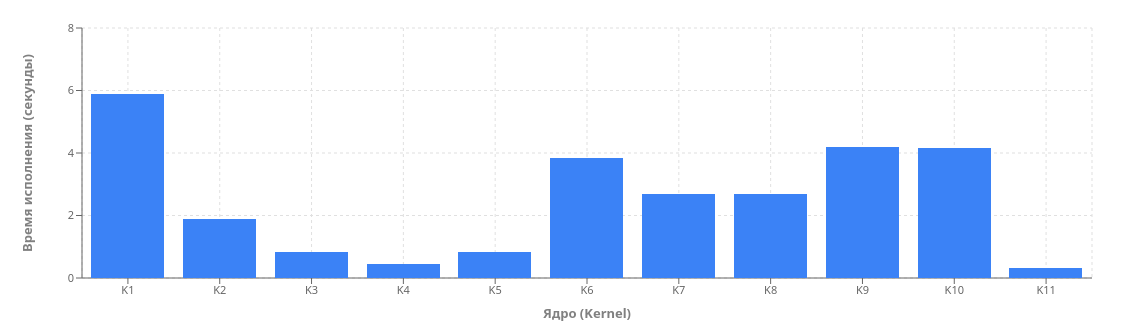
\includegraphics[width=0.95\textwidth]{figures/banana_pi_83232.png}
\caption{Производительность ядер MyGEMM на платформе Banana Pi BPI-F3 для конфигурации TS=8, TSM=32, TSN=32}
\label{fig:perf_bananapi}
\end{figure}

\begin{figure}[ht]
\centering
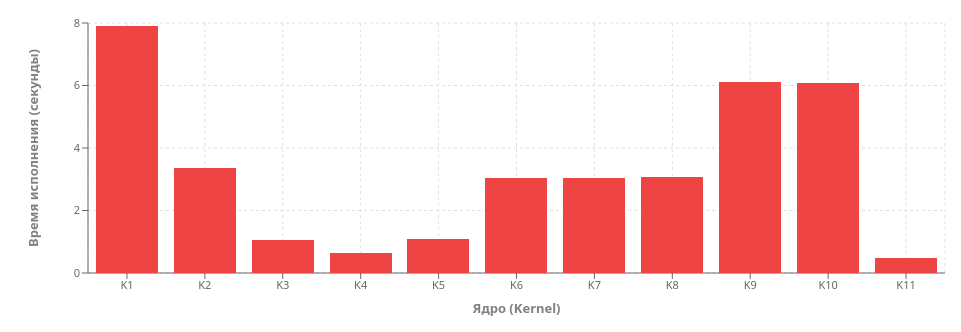
\includegraphics[width=0.95\textwidth]{figures/starfive_83232.png}
\caption{Производительность ядер MyGEMM на платформе StarFive VisionFive 2 для конфигурации TS=8, TSM=32, TSN=32}
\label{fig:perf_starfive}
\end{figure}

\begin{figure}[ht]
\centering
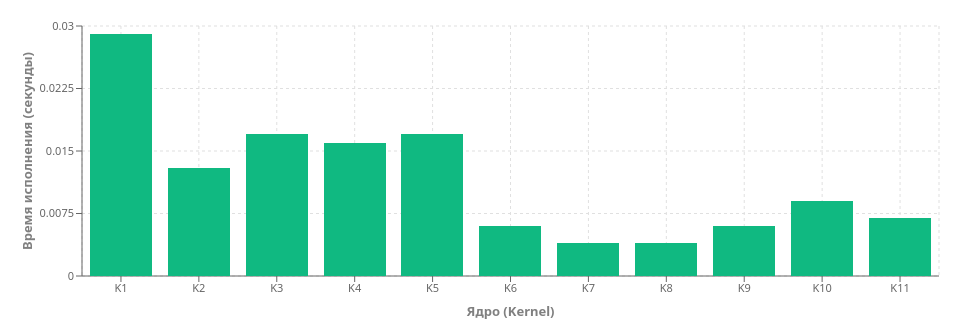
\includegraphics[width=0.95\textwidth]{figures/intel_xe_83232.png}
\caption{Производительность ядер MyGEMM на референсной платформе Intel Iris Xe для конфигурации TS=8, TSM=32, TSN=32}
\label{fig:perf_intelxe}
\end{figure}

\subsubsection{Анализ результатов}

Экспериментальные данные демонстрируют значительные различия в производительности между RISC-V платформами и референсной системой Intel Xe. Референсная платформа Intel Xe показывает время выполнения в диапазоне 0.004--0.029 секунд для различных ядер, что в среднем в 200--400 раз быстрее, чем RISC-V платформы.

Среди RISC-V платформ Banana Pi BPI-F3 демонстрирует лучшую производительность по сравнению со StarFive VisionFive 2, что объясняется более высокой тактовой частотой (2.0 ГГц против 1.5 ГГц) и большим количеством вычислительных ядер (8 против 4). Среднее время выполнения на Banana Pi составляет 0.3--11 секунд, на StarFive -- 0.5--9 секунд.

Ключевые наблюдения:
\begin{itemize}
    \item \textbf{Наилучший результат}: Ядро 11 (clBLAS-подход) демонстрирует наилучшую производительность на всех трёх платформах. На Banana Pi время выполнения составляет 0.32 сек, на StarFive -- 0.49 сек, на Intel Xe -- 0.007 сек. Это ядро не использует локальную память и полностью полагается на регистровую блокировку с векторными типами данных.
    
    \item \textbf{Проблемы векторизации}: Ядра 6--10, активно использующие векторизацию загрузки/записи данных, показывают неожиданно низкую производительность на RISC-V платформах. Время выполнения достигает 9--11 секунд, что в 10--30 раз медленнее более простых ядер 3--5. Это указывает на недостаточную оптимизацию драйверов OpenCL для векторных операций на архитектуре RISC-V.
    
    \item \textbf{Эффективность базовых оптимизаций}: Ядра 2--5, использующие блочную обработку с локальной памятью и work-per-thread оптимизацию, показывают хороший результат. Ядра 4 и 5 (2D регистровая блокировка с транспонированием) достигают времени 0.3--0.6 секунд на RISC-V, что в 10--25 раз быстрее наивной реализации (ядро 1).
    
    \item \textbf{Ограничения архитектуры}: Жёсткое ограничение размера рабочей группы в 32 потока на RISC-V платформах существенно ограничивает возможности оптимизации. Многие конфигурации параметров, эффективные на дискретных GPU, не могут быть использованы на RISC-V.
\end{itemize}

Полученные результаты показывают, что для достижения приемлемой производительности на RISC-V платформах следует отдавать предпочтение подходу, реализованному в ядре 11 (clBLAS), который не использует локальную память и основывается на регистровой блокировке. Ядра с активной векторизацией (6--10) следует избегать до улучшения драйверов OpenCL.

\printbibliography[heading=bibintoc,title={Список литературы}]

\end{document}